\chapter{Grundlagen}\label{chp:Grundlageb}
Im diesen Kapitel werden die theoretischen Grundlagen der Masterarbeit beschrieben, die zum Verst�ndnis der nachfolgenden Kapitel notwendig sind. Zu Beginn wird ein �berblick der Hintergrundsubtraktion gegeben und aufgezeigt, welche Besonderheiten diese Arbeit auszeichnen. An schlie�end wird die Histogrammanalyse zur Erkennung der K�rperhaltung erl�utert. Zuletzt befasst der letzte Teil sich mit einem �berblick �ber das wichtiges Framework OpenCV, das f�r moderne Computer Vision entwickelt wird. 
%%%%%%%%%%%%%%%%%%%%%%%%%%%%%%%%%%%%%%%%%%%%%%%%%%%%%%%%%%%%%%%%%%%%%%%%%%%%%%%%%%%%%%%%%%%%%%%
\section{Hintergrundsubtraktion}\label{sec:Grundlage1}
Die Hintergrundsubtraktion ist eine gebr�uchliche und weit verwendete Technik unter Verwendung von statischen Kameras zum Erzeugen eines Bin�rbildes, das die Pixel enth�lt, die zu sich bewegenden Objekten in der Szene geh�ren. Wie der Name andeutet, berechnet Hintergrundsubtraktion die Vordergrundmaske, die eine Subtraktion zwischen dem aktuellen Bild und einem Hintergrundmodell durchf�hrt, wobei der statische Teil der Szene oder allgemeiner alles, was angesichts der Merkmale der beobachtete Szene als Hintergrund betrachtet werden kann, enthalten ist.\\
In der Arbeit \cite{benezeth2010comparative} wird eine vergleichende Studie verschiedener Hintergrundsubtraktionsverfahren nach dem Stand der Technik pr�sentiert. Dieses Verfahren wurde seit den 1990er umfassend untersucht und haupts�chlich f�r Video�berwachungsanwendungen, da sie zuerst Personen, Fahrzeuge, Tiere usw. erkennen m�ssen, bevor komplexere Prozesse zur Einbruchserkennung, Verfolgung, Personenz�hlung \cite{aziz2011pedestrian} usw. ausgef�hrt werden. Viele Algorithmen wurden entworfen, um die Vordergrundobjekte vom Hintergrund einer Sequenz zu segmentieren und teilen im Allgemeinen das gleiche Schema:

\begin{itemize}
	\item Initialisierung des Hintergrundes: Ein Hintergrundmodell wird zuerst dank einer festen Anzahl von Frames zu bauen. Dieses Modell kann auf verschiedene Arten entworfen werden (statistisch, Fuzzy...)
	\item Erkennung des Vordergrundes: In den n�chsten Frames wird ein Vergleich zwischen dem aktuellen Frame und dem Hintergrundmodell durchgef�hrt. Diese Subtraktion f�hrt zu Berechnung des Verdergrundes der Szene.
	\item Initialisierung des Hintergrundes: W�hrend dieses Erfassungsprozesses werden auch Bilder analysiert, um das im Initialisierungsschritt gelernte Hintergrundmodell in Bezug auf eine Lernrate zu aktualisieren. Ein Objekt, das sich nicht lange bewegt, sollte im Hintergrund integriert sein.
\end{itemize}

\begin{figure}[htpb]
	\centering
	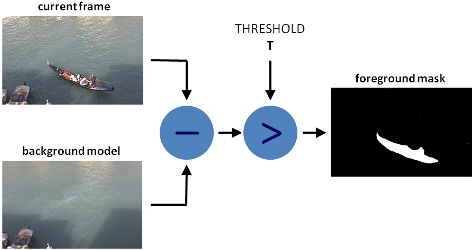
\includegraphics[width=0.90\textwidth]{fig/BS_Example.png}
	\caption{Ein Beispiel f�r Hintergrundsubtraktion }
	\label{fig:BS_Example}
\end{figure}
Im n�chsten Teil werden verschiedene state-of-art Verfahren beschrieben, um dies Verfahren genauer zu verstehen, wie die Hintergrundsubtraktion funktionieren soll.
\subsection{Gau�schen Mixture Modell}
In \cite{kaewtrakulpong2002improved} ist das entwickelte Hintergrundmodell auf der Grundlage der Gau�'schen Mischung pr�sentiert, das ein meist gebr�uchliche Weg ist. Es verwendet eine Methode, um jedes Hintergrundpixel durch eine Mischung von K-Gau�schen Verteilung (normalerweise K = 3 bis 5) zu modellieren. Die Gewichte der Mischung stellen die Zeitanteile dar, die diese Farbe in der Szene verbleiben. Die wahrscheinlichen Hintergrundfarben sind diejenigen, die l�nger und statischer bleiben \cite{kaewtrakulpong2002improved}.\\
Jedes Pixel in der Szene wird durch eine Mi schung von K-Gau�schen Verteilung modelliert. Die Wahrscheinlichkeit, dass ein bestimmtes Pixel zum Zeitpunkt $N$ einen Wert von $\mathrm{x}_{n}$ hat, kann wie folgt geschrieben werden:\\
\begin{equation}
p(\mathrm{x}_{n}) = \sum \limits_{j=1}^K w_j \eta(\mathrm{x}_{n};\theta_j)
\end{equation}
wobei $w_k$ ist Gewichtsparameter der k-ten Gau�-Komponente ist. $\eta(\mathrm{x}_{n};\theta_j)$ ist die Normalverteilung der k-ten Komponente, die wie folgt dargestellt wird \cite{kaewtrakulpong2002improved}:\\
\begin{equation}
\eta(\mathrm{x};\theta_j) = \eta(x;\mu_k, \Sigma_k) = \frac{1}{(2\pi)^\frac{D}{2} |\Sigma_k|^\frac{1}{2}} \mathrm{e}^{-\frac{1}{2}(x-\mu_k)^T \Sigma_k^{-1}(x-\mu_k)}
\end{equation}
wobei $\mu_k$ der Durchschnitt ist und $\Sigma_k =  \sigma^2_k I$ ist die Kovarianz der k-ten Komponente \cite{kaewtrakulpong2002improved}. Die K-Verteilungen sind auf der Grundlage des Fitnesswerts $\frac{w_k}{\sigma_k}$ geordnet und die ersten $B$-Verteilungen werden als ein Modell des Hintergrundes der Szene verwendet, wo $B$ wie folgt beschrieben werden:\\
\begin{equation}
B = \underset{b}{\arg\min}(\sum \limits_{j=1}^b w_j > T) 
\end{equation}
Und das Schwellwert $T$ ist Mindestanteil des Hintergrundmodells, n�mlich ist $T$ das minimale Wahrscheinlichkeit, dass der Hintergrund in der Szene ist. Die Hintergrundsubtraktion wird durchgef�hrt, indem ein Vordergrundpixel jedes Pixel markiert wird, das mehr als 2,5 Standardabweichungen von irgendeiner der B-Verteilung  entfernt ist. Die erste Gau�-Komponente, die die oben genannte Bedingung erf�llt, wird durch die folgenden Aktualisierungsgleichungen aktualisiert \cite{kaewtrakulpong2002improved}:
\begin{eqnarray}
\hat{w}^{N+1}_k &=& (1-\alpha) \hat{w}^{N}_k + \alpha \hat{p} (w_k | \mathrm{x}_{N+1}) \\
\hat{\mu}^{N+1}_k &=& (1-\alpha) \hat{\mu}^N_k + \rho\mathrm{x}_{N+1} \\
\hat{\Sigma}^{N+1}_k &=& (1-\alpha)\hat{\Sigma}^N_k + \rho(\mathrm{x}_{N+1} - \hat{\mu}^{N+1}_k)(\mathrm{x}_{N+1} - \hat{\mu}^{N+1}_k)^T\\
\rho &=& \alpha\eta(\mathrm{x}_{N+1};\hat{\mu}^N_k; \hat{\Sigma}^N_k)\\
 X&=&\left\{\begin{array}{@{}ll@{}}
0, & \text{wenn}\ w_k\ \text{erste Gau�-Komponente ist} \\
1, & \text{sonst}
\end{array}\right.
\end{eqnarray}
wobei $w_k$ die k-ten Gau�schen Komponente und $\frac{1}{\alpha}$ definiert die Zeitkonstante, die die �nderung bestimmt. Wenn keine der K-Verteilung mit diesem Pixelwert �bereinstimmt, wird die unwahrscheinliche Komponente durch eine Verteilung mit dem aktuellen Wert als Mittelwert ersetzt.

\subsection{Adaptive Gau�schen Mixture Modell}
In \cite{zivkovic2006efficient} wurde eine interessante Erweiterung von GMM vorgeschlagen. Normales GMM wird mit eine bestimmte Anzahl von Gau�schen Modell, aber AGMM wird automatisch die Anzahl der Gau�schen Variablen angepasst, die zur Modellierung eines gegebenen Pixels verwendet werden. Die Erweiterung reduziert die Speicheranforderung des Algorithmus, erh�ht die Recheneffizienz und kann die Leistung verbessern, wenn der Hintergrund stark sich �ndert.

 


\section{Histogrammanalyse}
Wie schon in Kapitel~\ref{sec:Grundlage1} beschrieben ...
\section{OpenCV Framework}\label{sec:OpenCV}
text